\section{Retrieval of Medical Guidelines}
\subsection{NICE API}
After applying for access to use the NICE API to save guideline on device to enable the retrieval of medical guidelines, we discussed our approach with a representitive from their security team. He expressed the limitations that would be imposed on the project if the original plan of storing all medical guidance on device was undertaken. The NICE security team only allows access of their content through the API, and must guarantee that NICE information cannot be accessed outside of the UK. As a result, the only acceptable solution would require an API key to be hosted on either a private UCL or NHS network. This would break the core principle of an offline solution. After collaborating with my supervisors, we shifted our approach. 

\subsection{Design}
Instead of a purpose build RAG for NICE guidelines, the application would support the uploading of medical guidance PDF's from the doctor's file system. This guidance would be queried to highlight relevant medical guidelines based on the summarisation.

\subsubsection{Pipeline}
The pipeline operates in 2 phases: indexing on user upload and querying when searching for guidelines
\begin{itemize}
    \item \textbf{Indexing} \texttt{GuidelineIndexer.cpp}: a PDF is parsed by MuPDF into structured text blocks, then each block is embedded with MedCPT, and the resulting vector is inserted into an HNSW graph. The chunk's metadata (PDF name, page number, bounding box, raw text) is written to an SQLite table keyed by an autoincrementing chunk identifier. The same identifier is used as the HNSW node label so that a vector hit can be resolved back to its source passage.
    \item \textbf{Querying} \texttt{GuidelineRAG.cpp}: the consultation summary is embedded with the same MedCPT model, the embedding is L2-normalised, and an HNSW ANN search returns the top 5 chunk identifiers. Each identifier is resolved against the SQLite database to produce a \texttt{GuidelineResult} record. Finally, the results are sorted by L2 distance before being returned to the UI.
\end{itemize}

\subsubsection{Error Handling}
As the SQLite database is packaged empty, all libraries and models are packaged with the application, and all uploaded PDFs are copied into the sandbox environment, the only point of failure is the uploading of PDFs. To handle this, the file explorer popup only accepts PDF files to prevent invalid file upload to the application.

\subsubsection{Chunking Strategy}
Although a naive token window chunking method would provide uniform vectors and simple implementation, it could split logically related passages and treat PDF artefacts such as page numbers, headers and footnotes as valid chunks. This evaluation resulted in the current design; delegating chunking to MuPDF's structural text extractor, returning logical text blocks segmented by the PDF's layout. Blocks containing fewer than 5 words are filtered to remove page numbers, headers and footers. Although the chunks produced vary in length, they are semantically coherent and avoid potential matches against PDF artefacts.

The HNSW graph persists alongside the SQLite database in a \texttt{nice\_guidelines.bin} file which holds the embeddings tree. Any PDF files uploaded by the user will be copied into the MSIX sandbox to ensure external file movement is isolated from the application.

\subsubsection{ANN Search}
HNSWLib's hierarchical navigable small worlds index gives sub-linear search time at the cost of a small recall drop relative to exact $k$-NN searches. This trade-off is acceptable for clinical guidance retrieval, where the system is surfacing candidate passages for human review rather than answering definitively. Furthermore, as documents of any size can be added and removed at any time, the latency of embedding and searching is crucial to the application's usability. 

\subsection{Implementation}
\subsubsection{Incompatability}
Although the design called for the MedCPT model to be ran on the NPU, there were implementation issues. After extensive debugging, a root cause for the model failing to load and crash the application could not be found. After consulting my external supervisor, using the NPU was de-prioritised due to a CPU implementation resulting in acceptable inference latency.

\subsubsection{Concurrency}
\texttt{GuidelineRAG::Initialize()} runs on its own background thread spawned during application start (\texttt{m\_ragLoadFuture}), parallel to the summarisation engine load. Indexing operations are dispatched from the UI thread to a worker via \texttt{std::async} so PDF parsing and embedding never block UI updates. Queries run on a short lived worker thread spawned when the user selects \emph{View Guidance}. There is no shared mutable state between concurrent queries, so no explicit locking is required.

\subsubsection{Storage}
The retrieved passages must point back to a precise location in the source PDF so that the UI can highlight them in an embedded MuPDF viewer. To support this without re-parsing the document at query time, the indexer stores both the chunk text and its bounding box on the page:

\begin{verbatim}
CREATE TABLE IF NOT EXISTS guidelines (
    chunk_id       INTEGER PRIMARY KEY,
    guideline_name TEXT,
    page_number    INTEGER,
    bbox_x0 REAL, bbox_y0 REAL,
    bbox_x1 REAL, bbox_y1 REAL,
    chunk_text     TEXT
);
\end{verbatim}

Because the application runs inside the MSIX sandbox, the SQLite connection sets \texttt{PRAGMA journal\_mode = MEMORY} avoiding sandbox-incompatible journal files and \texttt{PRAGMA synchronous = NORMAL} preserving durability of metadata writes.

\subsubsection{Indexing a PDF}
\begin{enumerate}
    \item Open the document via \texttt{fz\_open\_document()}; iterate pages, extract structured text via \texttt{fz\_new\_stext\_page\_from\_page()} and walk the \texttt{block $\rightarrow$ line $\rightarrow$ char} hierarchy, encoding non-ASCII characters as UTF-8.
    \item For each surviving block (more than five words), build the chunk text and bounding box.
    \item Embed the chunk via \texttt{GuidelineRAG::EmbedText()}, which tokenises the text, runs MedCPT, extracts the CLS-token output and L2-normalises it.
    \item Insert the embedding into the HNSW graph at a freshly allocated chunk identifier, then insert the chunk row into SQLite within a single transaction. The chunk identifier is shared between the two stores so that an HNSW hit can be resolved with one lookup.
    \item After commit, count the rows for the new \texttt{guideline\_name}; if the row count does not match the number of chunks added to HNSW, the entire index is rolled back. This caught a real failure mode where a partial write to SQLite (caused by an unrelated MSIX file-system limitation early in development) had left the HNSW graph and SQLite metadata out of sync.
\end{enumerate}

\subsubsection{UI}
Embedding the PDF file within the user interface allows for a native PDF viewing experience. The found guidance on the left jumps the user to the corresponding highlighted bounding box within the PDF viewer, and tabs across the top enable navigation between multiple PDFs
\begin{figure}
    \centering
    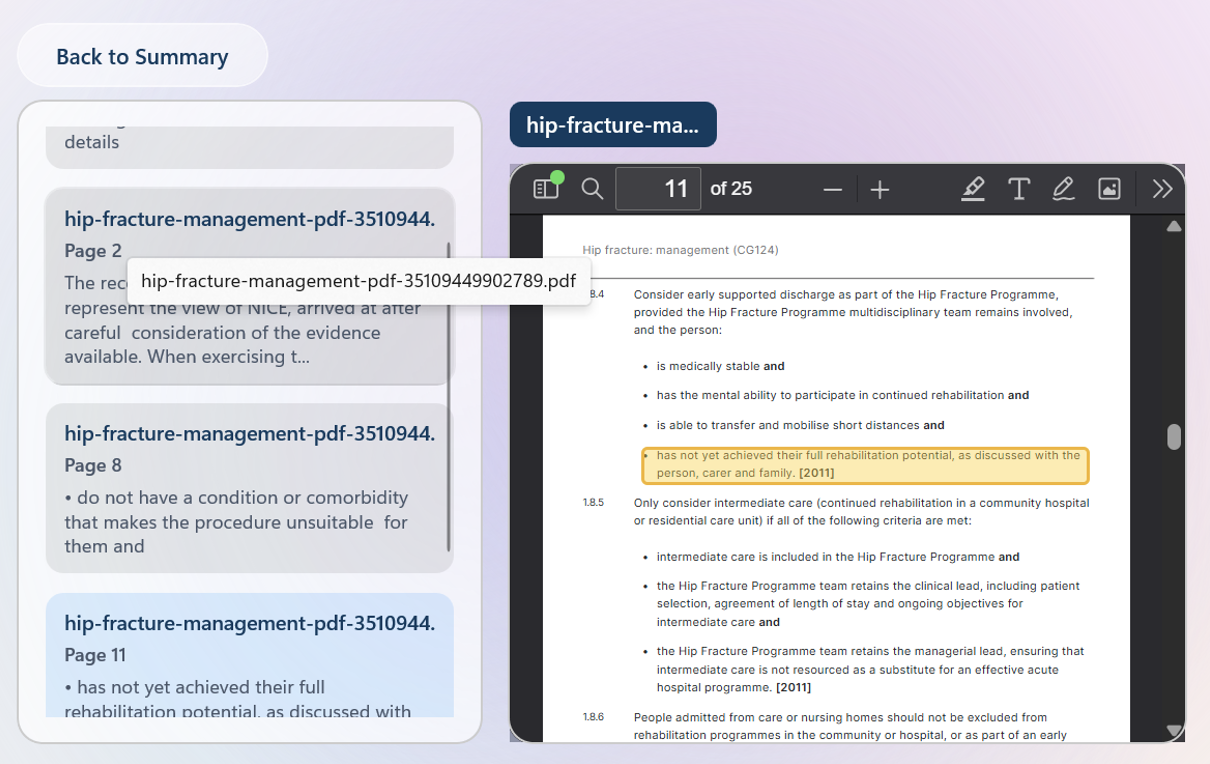
\includegraphics[width=0.5\linewidth]{uirag.png}
    \caption{User Interface for the retrieved guidelines based on a summarisation}
    \label{fig:uirag}
\end{figure}
